\begin{frame}{Disturbance Estimation}
	 \textbf{Objectives with the use of disturbance estimation}
	 \begin{itemize}
	 	\item VF-LQR controller needs an estimate of the consumer demand.
	 	\item The optimal estimator is the \textbf{Kalman Filter}.
	 \end{itemize}
\end{frame}

%%%%%%%%%%%%%%%%%

\begin{frame}{Disturbance Estimation}{The Kalman Filter}
 	\begin{itemize}
 		\item Need a linear model of consumer behaviour for the Kalman Filter
 		\item Under normal circumstances the Kalman gain is found recursively.
 		\item In the case of LTI system the Kalman filter itself becomes time invariant $\rightarrow$ constant Kalman gain.\\
 		ARE:
 		\begin{equation}
 			\begin{split}\label{eq:ss_kalman_udledning4}
 				&\Pi = {A} (\Pi^{-1} + {C}^T {R}^{-1} {C})^{-1} {A}^T + {Q}\\
 				& K = \Pi {C}^T ({C} \Pi {C}^T + {R})^{-1}
 			\end{split}
 		\end{equation}
 		\item Kalman filter is also very interesting from a leakage detection POV.
 	\end{itemize}
\end{frame}

%%%%%%%%%%%%%%%%%

\begin{frame}{Disturbance Estimation}{Water Consumption Data}
	\begin{itemize}
		\item Data of consumption pattern over a 35 day period courtesy of CSK and Grundfos.  
	\end{itemize}
		 \begin{figure}[h!]
			\centering
			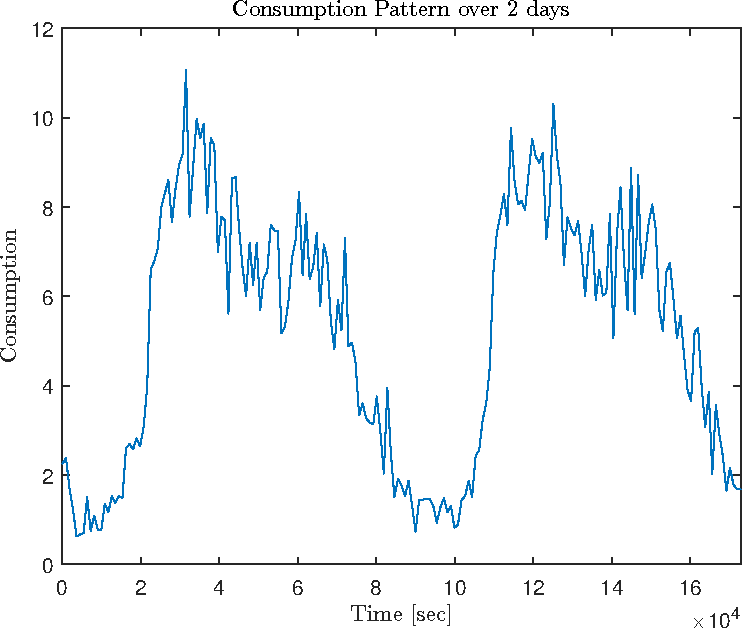
\includegraphics[width=0.6\textwidth]{Topics/KalmanEstimator/Graphics/ConsumptionPattern.pdf}
			\caption{Consumption pattern over two days}
			\label{fig:Consumption_Pattern}
		\end{figure}
\end{frame}

%%%%%%%%%%%%%%%%%
	
\begin{frame}{Disturbance Estimation}{FFT of Consumption Pattern}
	\begin{itemize}
		\item Frequency analysis of the data. 
	\end{itemize}
	
	 \begin{figure}[h!]
		\centering
		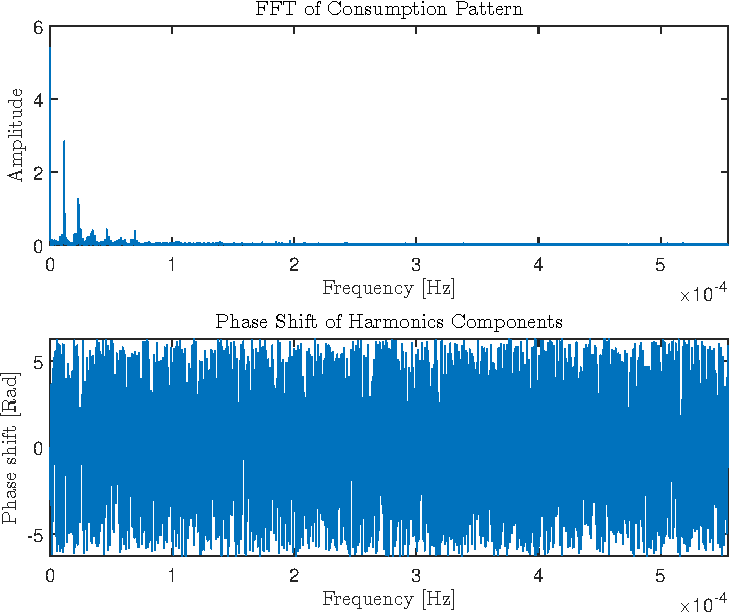
\includegraphics[width=0.6\textwidth]{Topics/KalmanEstimator/Graphics/FFT.pdf}
		\caption{Amplitude and phase content of full consumption pattern}
		\label{fig:FFT_Consumption_Patter}
	\end{figure}
	
 We want a sparse representation. Largest frequency components are: DC, $24.05 \text{hr}$, $12.03 \text{hr}$, $8.02 \text{hr}$ and $5.99 \text{hr}$.

\end{frame}

%%%%%%%%%%%%%%%%%
\begin{frame}{Disturbance Estimation}{Approximation of Consumption}
		
	\begin{itemize}
		\item Fourth-order Fourier approximation of consumer demand:
	\end{itemize}
		
	\begin{equation} \label{eq:4th_order_approx}
		\begin{split}
			d_c(t) \approx& k_0 + k_1 cos(\omega_1 t + \phi_1) + k_2 cos(\omega_2 t + \phi_2)\\
			&+ k_3 cos(3\omega_3 t + \phi_3) + k_4 cos(4\omega_4 t + \phi_4)
		\end{split}
	\end{equation}

	\begin{itemize}
		\item We wish to model equation \ref{eq:4th_order_approx} as a state-space model:
	\end{itemize}
		
		\begin{equation*}
		\begin{split}
			\dot{x}=Ax\\
			y=Cx
		\end{split}
		\end{equation*}	
\end{frame}

%%%%%%%%%%%%%%%%%%%%%%%

\begin{frame}{Disturbance Estimation}{State-space Representation}
	\begin{itemize}
		\item Need to represent the evolution of the "states" in the approximation as a linear combination of states.
		\item This can not be achieved using the current states.   
	\end{itemize}
	
\begin{equation} \label{eq:consump_A}
	\dot{x} = 
	\begin{bmatrix}
		0 & 0 & 0 & 0 & 0 \\
		0 & 0 & -\omega_1 & 0 & 0 \\
		0 & \omega_1 & 0 & 0 & 0 \\
		0 & 0 & 0 & 0 & -\omega_2 \\
		0 & 0 & 0 & \omega_2 & 0 
	\end{bmatrix}
	\begin{bmatrix}
		k_0 \\
		k_1 cos(\omega_1 t) \\
		k_1 sin(\omega_1 t) \\
		k_2 cos(\omega_2 t) \\
		k_2 sin(\omega_2 t) 
	\end{bmatrix}
\end{equation}

\begin{equation}
	C = \begin{bmatrix} 1 & 1 & 0 & 1 & 0 \end{bmatrix}, \quad 
	\dot{x} = \begin{bmatrix}0 \\ -k_1\omega_1sin(\omega_1 t) \\ k_1\omega_1 cos(\omega_1 t) \\ -k_2\omega_2sin(\omega_2 t) \\ k_2\omega_2 cos(\omega_2 t)  \end{bmatrix} 
\end{equation}

	\begin{itemize}
	\item Fourth order doesn't fit the page!
\end{itemize}
\end{frame}

%%%%%%%%%%%%%%%%%%%%%%%

\begin{frame}{Disturbance Estimation}{Model vs. Data}
	\begin{itemize}
			\item The model compared to the real data - shown over 2 days. 
	\end{itemize}
		\begin{figure}[h!]
			\centering
			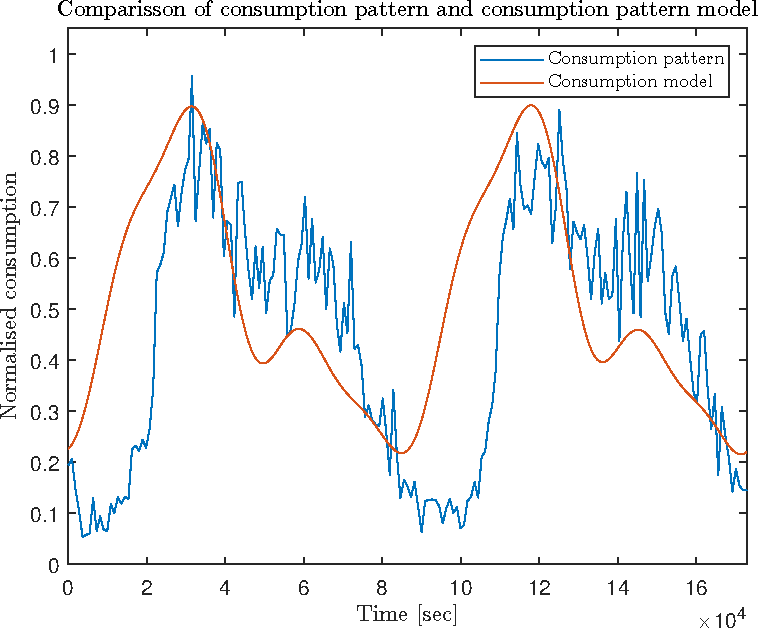
\includegraphics[width=0.6\textwidth]{Topics/KalmanEstimator/Graphics/Comparisson.pdf}
			\caption{Comparison of raw historical data, and model}
			\label{fig:Comparison}
		\end{figure}
	\begin{itemize}
		\item The model follows the visual trend in real data.
	\end{itemize}	
\end{frame}

%%%%%%%%%%%%%%%%%%%%%%%

\begin{frame}{Disturbance Estimation}{Kalman Filter Design}
	\textbf{Considerations when designing the KF.}
	\begin{itemize}
		\item In practice the Kalman gain is found using lqr in matlab.
		\item Stiffness of the filter is decided by Q-R ratio.
		\item Big R means uncertainty concerning observation and that we trust model much $\rightarrow$ stiff filter.
	\end{itemize}
\end{frame}